\section{模型构建}
本研究构建了一个基于 Vision Transformer（ViT）编码器与 Transformer 解码器的端到端模型框架，旨在实现数学表达式图像（涵盖印刷体与手写体）的识别与 LaTeX 转换。

其中，ViT 编码器通过自注意力机制将图像处理任务转化为序列处理任务，对输入图像进行全局建模，深入挖掘符号的空间关系与语义特征，提升对复杂结构的感知能力；Transformer 解码器则基于自注意力和交叉注意力机制，分别建模生成序列的内部依赖和编码图像与解码序列之间的对齐，从而实现对 LaTeX 序列的高质量生成。

该框架将视觉特征提取与序列生成统一于端到端结构中，便于对图像编码与 LaTeX 解码两个阶段进行联合优化。
\subsection{数据来源与预处理}
\subsubsection{数据来源}
本研究以数学表达式的结构识别与 LaTeX 转换为目标任务。考虑到方法验证需要结构清晰、标注规范且被广泛用作基准的数据集，本文选用印刷体数学表达式数据集 \texttt{im2latex-100k}\supercite{kanervisto_2016_56198} 作为主要训练与评估数据集：该数据集格式规范、规模充足，便于与现有方法进行横向对比，也便于将性能差异归因于模型本身而非数据噪声。

针对手写数学表达式这一目标应用场景，本文进一步选用手写体数据集 \texttt{MathWriting-human}\supercite{gervaisMathWritingDatasetHandwritten2025} 开展对比实验。该数据集收集了大量真实用户手写的数学表达式图像，具有较高的结构复杂性和风格多样性，更贴近实际应用场景。本文以与印刷体实验完全相同的模型架构与训练配方在该数据集上训练和评估，以考察方法向手写场景迁移的能力（见“结果与评价”一章的手写场景对比实验）。

如图~\ref{fig:dataset-samples} 所示，其中（a）（b）分别展示了手写体与印刷体数据集中具有代表性的样本图像。

\begin{figure}[H]
    \centering
    \begin{subfigure}[b]{0.48\textwidth}
        \centering
        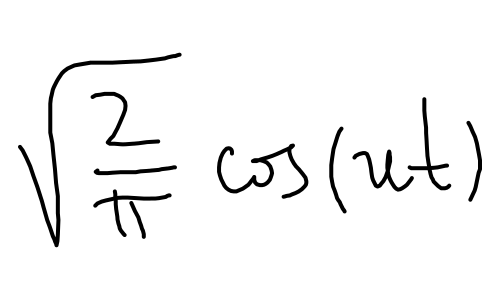
\includegraphics[width=0.9\linewidth, keepaspectratio]{pic/mathwriting-human-sample}
        \caption{\texttt{MathWriting-human} 手写体样本}
        \label{fig:mathwriting-human-sample}
    \end{subfigure}
    \hfill
    \begin{subfigure}[b]{0.48\textwidth}
        \centering
        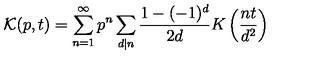
\includegraphics[width=0.9\linewidth, keepaspectratio]{pic/printed-math-expression}
        \caption{\texttt{im2latex-100k} 印刷体样本}
        \label{fig:printed-math-expression}
    \end{subfigure}
    \caption{两类数据集的代表性样本图像}
    \label{fig:dataset-samples}
\end{figure}

两个数据集的加载方式如下：
\begin{itemize}
    \item \texttt{MathWriting-human} 可通过 HuggingFace 平台获取\footnotemark[1]；
    \item \texttt{im2latex-100k} 可通过 HuggingFace 平台获取\footnotemark[2]。
\end{itemize}

\footnotetext[1]{\url{https://huggingface.co/datasets/deepcopy/MathWriting-human}；也可使用\texttt{datasets} 库命令 \texttt{load\_dataset("deepcopy/MathWriting-human")} 加载。}
\footnotetext[2]{\url{https://huggingface.co/datasets/yuntian-deng/im2latex-100k}；也可使用\texttt{datasets} 库命令 \texttt{load\_dataset("yuntian-deng/im2latex-100k")} 加载。}

本节余下内容基于 \texttt{im2latex-100k} 数据集详细介绍模型构建的完整流程。模型与数据处理流程基于 PyTorch 框架实现；该流程同样适用于 \texttt{MathWriting-human} 数据集，仅需根据具体情况对部分参数进行适当调整。下文以 $B$ 记批大小（本文实验中 $B=768$）。
\subsubsection{数据预处理}
本文对所采用的数学表达式数据集中的图像与文本数据均进行了标准化预处理操作，以提升模型训练效果与表达一致性。

图像处理主要包括尺寸规范化与像素归一化，文本处理则将 LaTeX 表达式转化为模型可读的标记序列。具体步骤如下所示：

\begin{enumerate}[label={（\arabic*）}, leftmargin=2em, labelsep=0.5em, itemsep=0pt]
\item 图像预处理：
\begin{enumerate}[label={（\alph*）}, leftmargin=2em, labelsep=0.5em, itemsep=0pt]
\item 通过 \texttt{datasets} 库载入训练数据，直接获取 PIL 格式的原始图像（RGB、尺寸不一）；
\item 将图像转换为灰度格式，通道数为 $1$；
\item 将图像统一缩放至尺寸 $50 \times 200$，并归一化像素值至 $[0,1]$ 区间；
\item 构建通道在前的图像批次张量（形状 $[B, 1, 50, 200]$），满足模型输入维度要求；
\end{enumerate}
\item 文本预处理：
\begin{enumerate}[label={（\alph*）}, leftmargin=2em, labelsep=0.5em, itemsep=0pt]
\item 载入训练数据，为每条 LaTeX 表达式添加特殊标记 \texttt{[START]} 与 \texttt{[END]}；
\item 词元规范化：\texttt{im2latex-100k} 的公式已是空格分隔的词元序列，直接按空白切分；\texttt{MathWriting-human} 的 \texttt{latex} 字段为未分词的原始字符串（如 \texttt{V(\textbackslash tilde\{\textbackslash beta\})}），先以正则规则切分为词元——LaTeX 命令（含星号形式，如 \texttt{\textbackslash operatorname*}）、转义符号（如 \texttt{\textbackslash\%}）各为一个词元，其余按单字符切分（数字逐位拆分，与 \texttt{im2latex} 约定一致）——再以空格连接，统一两个数据集的词元约定；
\item 构建基于训练语料的分词器（Tokenizer）：按空白切分词元、保留大小写与全部 LaTeX 符号，词表按词频降序构建并约定索引 $0$ 为填充符、索引 $1$ 为 \texttt{[UNK]}，确保转换过程中保留语义及语法信息；
\item 使用分词器将 LaTeX 表达式转换为整数索引序列，并后向填充至固定长度 $152$；
\end{enumerate}
\end{enumerate}
\subsection{编码器：Vision Transformer}
本文引入 Vision Transformer（ViT）作为编码器，以增强模型对手写数学表达式图像中复杂结构与全局语义的建模能力。
ViT 首先将输入图像划分为固定大小的图像块（patch），再将每个图像块展平并嵌入高维特征空间，构建图像块序列以供 Transformer 编码器处理。
得益于全局自注意力机制，ViT 能直接建模图像中远距离符号之间的依赖关系，不受卷积网络局部感受野的约束。

相比基于 CNN 的方法，ViT 在建模长程结构依赖方面更具优势，适用于结构复杂、符号排列多变的数学表达式图像。
其对图像空间结构的建模能力为解码器生成 LaTeX 序列提供了图像特征表示（生成质量见“结果与评价”一章）。

\subsubsection{序列化处理}
\begin{enumerate}[label={（\arabic*）}, leftmargin=2em, labelsep=0.5em, itemsep=0pt]
    \item 图像分块：将输入图像（$\texttt{IMG\_SHAPE}=[50, 200, 1]$）划分为 $\texttt{PATCH\_SIZE}=10 \times 10$ 的非重叠图像块，得到 $\texttt{NUM\_PATCHES}=(50 \div 10) \times (200 \div 10) = 100$ 个图像块，并重组为序列形式；
    \item 线性投影：将 $\texttt{NUM\_PATCHES}=100$ 个图像块组成的序列输入线性层，映射至维度为 $\texttt{EMBEDDING\_DIM}=256$ 的特征空间，获取图像块的高维表示；
    \item 位置编码：为每个图像块分配可学习的位置编码，采用 $[0, \cdots, \texttt{NUM\_PATCHES}-1]=[0, 1, \cdots, 99]$ 作为索引，以建模图像块在原图中的空间位置信息；
    \item 输入序列构建：将图像块特征与对应位置编码逐元素相加，组成输入序列，形状为 $[B, \texttt{NUM\_PATCHES}, \texttt{EMBEDDING\_DIM}] = [B, 100, 256]$，作为 Transformer 编码器的输入。
\end{enumerate}
注：如“Vision Transformer 基本原理”一章所述，序列生成任务使用编码器输出的全部图像块特征序列，而非面向分类的 [CLS] 全局表征。因此本文不引入“可学习类别标记”：编码器直接输出与 $100$ 个图像块一一对应的特征序列，作为解码器交叉注意力的键与值，由其完成视觉—文本对齐。该设计与目标任务的序列生成性质一致，同时避免了 [CLS] 标记引入的额外位置与计算开销。
\subsubsection{编码器架构}
\begin{enumerate}[label={（\arabic*）}, leftmargin=2em, labelsep=0.5em, itemsep=0pt]
    \item 层归一化：参数$\epsilon=10^{-6}$（代码中 \texttt{epsilon=1e-6}），对输入序列进行归一化处理，确保数值稳定性；
    \item 多头自注意力：采用 $\texttt{NUM\_HEADS}=4$ 个头的多头自注意力机制（\texttt{nn.MultiheadAttention}），总嵌入维度 $\texttt{EMBEDDING\_DIM}=256$ 平均分配至各头，每头维度为 $256 \div 4 = 64$；注意力权重的 Dropout 概率为 $\texttt{DROPOUT\_RATE}=0.1$；
    \item 残差连接：将多头自注意力的输出与输入序列相加，形成残差连接，增强梯度流动；
    \item 层归一化：参数$\epsilon=10^{-6}$（代码中 \texttt{epsilon=1e-6}），对残差连接进行归一化处理，确保数值稳定性；
    \item 多层感知机（MLP）：由两个线性层构成（$256 \to 512 \to 256$），每个线性层之后均接 GELU 激活与 Dropout（概率 $\texttt{DROPOUT\_RATE}=0.1$），整体呈扩展—收缩结构，其中：
    \begin{itemize}
        \item 扩展阶段：线性层 $\texttt{nn.Linear(256, 512)}$ 将特征由 $\texttt{EMBEDDING\_DIM}=256$ 维升至 $512$ 维，随后经 GELU 激活与 Dropout，以增强非线性表达能力（GELU 相比 ReLU 梯度更平滑，有利于训练稳定）；
        \item 收缩阶段：线性层 $\texttt{nn.Linear(512, 256)}$ 将特征降回 $\texttt{EMBEDDING\_DIM}=256$ 维，同样经 GELU 激活与 Dropout，使输出维度与输入一致，便于残差连接；
        \item 设计原理：扩展-收缩模式遵循标准Transformer架构，通过先扩展后收缩的方式，在保持输入输出维度匹配的同时，增强非线性表达能力。
    \end{itemize}
    \item 残差连接：将 MLP 输出与第一个残差连接的输出相加，形成第二个残差连接，进一步增强梯度流动；
\end{enumerate}
将上述结构重复 $\texttt{TRANSFORMER\_LAYERS}=8$ 次，形成深度Transformer编码器，增强模型的表达能力。
随后对最后一个Transformer块的输出进行最终层归一化处理（$\texttt{epsilon=1e-6}$），确保特征表示的数值稳定性。
最终输出：经过 $8$ 层Transformer块处理和最终归一化后的特征表示，形状为 $[B, \texttt{NUM\_PATCHES}, \texttt{EMBEDDING\_DIM}]=[B, 100, 256]$，其中 $\texttt{NUM\_PATCHES}=(50 \div 10) \times (200 \div 10) = 100$。

\subsection{解码器：Transformer}
本文采用标准的 Transformer 解码器结构，将编码器提取的图像表示自回归地映射为结构化的 LaTeX 序列。该解码器融合自注意力与交叉注意力机制，协同建模目标序列的内部依赖与图像特征之间的对应关系。

其中，交叉注意力机制通过引导解码器聚焦于编码器输出中与当前生成阶段最相关的图像区域特征，提升视觉-语言对齐效果；
而自注意力机制则用于捕捉目标序列内部的依赖关系，确保解码过程中的上下文一致性与语义连贯性。
该双重注意力结构旨在同时建模目标序列的内部依赖与图像—文本对齐关系，为高质量的 LaTeX 序列生成提供结构支撑（实际效果见“结果与评价”一章）。

\subsubsection{解码器架构}
\begin{enumerate}[label={（\arabic*）}, leftmargin=2em, labelsep=0.5em, itemsep=0pt]
    \item 序列嵌入层（SeqEmbedding）：
        \begin{enumerate}[label={（\alph*）}, leftmargin=2em, labelsep=0.5em, itemsep=0pt]
            \item 词元嵌入：将输入的词元 ID转换为向量表示，维度为$\texttt{EMBEDDING\_DIM}=256$，并与可学习的位置编码逐元素相加融合；
            \item 填充处理：嵌入层指定 $\texttt{padding\_idx}=0$，将填充符的嵌入向量固定为零且不参与梯度更新；填充位置对优化目标的影响则由掩蔽损失函数（见“训练原理”一章）予以排除；
            \item 位置编码采用可学习的嵌入方式（$\texttt{nn.Embedding(max\_length, depth)}$），最大序列长度为$\texttt{MAX\_SEQ\_LEN\_1}=151$；为防止位置索引越界，解码前对输入序列统一截断至该长度。
        \end{enumerate}
    \item 因果自注意力层（CausalSelfAttention）：
        \begin{enumerate}[label={（\alph*）}, leftmargin=2em, labelsep=0.5em, itemsep=0pt]
            \item 输入为解码器当前的嵌入序列，设动态序列长度为\texttt{seq\_length}，则其形状为$[B, \texttt{seq\_length}, \texttt{EMBEDDING\_DIM}] = [B, \texttt{seq\_length}, 256]$：
                \begin{itemize}
                    \item 训练阶段：教师强制下取 $\texttt{sequences[:, :-1]}$ 作为输入，$\texttt{seq\_length}$ 固定为 $\texttt{MAX\_SEQ\_LEN\_1}=151$，填充位置由掩蔽损失从优化目标中排除；
                    \item 推理阶段：$\texttt{seq\_length}$ 从 $1$（仅含 $\texttt{[START]}$）开始，随自回归生成逐词元增长，直至生成 $\texttt{[END]}$ 或达到 $\texttt{MAX\_SEQ\_LEN\_1}=151$。
                \end{itemize}
            \item 使用因果掩码：构造上三角布尔矩阵作为注意力掩码（$\texttt{torch.triu}$，对角线以上为屏蔽位置），确保解码器只能查看到已经生成的部分，并避免信息泄漏；
            \item 使用残差连接和层归一化（本文解码器采用 Post-LN，即先残差相加再归一化 $\text{LayerNorm}(\boldsymbol{x}+\text{Sublayer}(\boldsymbol{x}))$，与编码器的 Pre-LN 相对），增强梯度流动和训练稳定性；
            \item 采用 $\texttt{DECODER\_HEADS}=8$ 头的多头注意力机制，总嵌入维度 $256$ 平均分配至各头，每头维度为 $256 \div 8 = 32$。
        \end{enumerate}
    \item 交叉注意力层（CrossAttention）：
\begin{enumerate}[label={（\alph*）}, leftmargin=2em, labelsep=0.5em, itemsep=0pt]
    \item 查询为文本序列，键与值为图像特征序列，输出为融合了图像信息的文本隐藏表示（并非最终 LaTeX 序列，后者还需经前馈层与输出层进一步生成）；
    \item 图像特征形状为$[B, \texttt{NUM\_PATCHES}, \texttt{EMBEDDING\_DIM}] = [B, 100, 256]$（基于$\texttt{IMG\_SHAPE}=[50, 200, 1]$图像和$\texttt{PATCH\_SIZE}=10 \times 10$的图像块大小），文本序列形状为$[B, \texttt{seq\_length}, 256]$，其中：
    \begin{itemize}
        \item 图像特征：来自ViT编码器的输出，包含$100$个图像块的特征表示，每个图像块对应图像中的一个$10 \times 10$区域；
        \item 文本序列：来自解码器的当前嵌入状态，长度$\texttt{seq\_length}$为动态值；
        \item 跨模态融合：以文本序列为查询（Query）、图像特征为键与值（Key/Value）调用多头注意力（$\texttt{mha(x, y, y)}$），实现文本对图像特征的注意力机制。
    \end{itemize}
    \item 使用残差连接与层归一化；并保存交叉注意力分数（形状 $[B, \texttt{seq\_length}, \texttt{NUM\_PATCHES}]$，各头取平均）用于可视化，以分析生成各词元时模型关注的图像区域。
\end{enumerate}
\item 前馈网络层（FeedForward）：
\begin{enumerate}[label={（\alph*）}, leftmargin=2em, labelsep=0.5em, itemsep=0pt]
    \item 由两个线性层构成（单个隐藏层，维度 $\texttt{EMBEDDING\_DIM} \times 2 = 512$；输出维度回到 $\texttt{EMBEDDING\_DIM} = 256$），采用扩展-收缩结构，其中：
    \begin{itemize}
        \item 第一层：$\texttt{nn.Linear(256, 512)}$，使用ReLU激活函数，将输入特征从256维扩展至512维，增强模型的非线性表达能力；
        \item 第二层：$\texttt{nn.Linear(512, 256)}$，无激活函数（线性激活），将特征维度收缩回256维，保持与输入维度一致，便于残差连接；
        \item Dropout层：概率为$\texttt{DROPOUT\_RATE}=0.1$，在训练时随机丢弃部分神经元激活，防止过拟合并增强模型泛化能力。
    \end{itemize}
\end{enumerate}
    \item 解码器层（DecoderLayer）：
        \begin{enumerate}[label={（\alph*）}, leftmargin=2em, labelsep=0.5em, itemsep=0pt]
            \item 共三个子层：因果自注意力层、交叉注意力层和前馈网络层，其中两个注意力子层均采用 $\texttt{DECODER\_HEADS}=8$ 头的多头注意力机制，其中：
            \begin{itemize}
                \item 因果自注意力：处理文本序列内部依赖关系，使用上三角因果掩码确保每个位置只能访问之前的位置，防止信息泄漏；
                \item 交叉注意力：实现文本对图像特征的注意力机制，其中文本序列作为查询、图像特征作为键值对，实现跨模态信息融合；
                \item 前馈网络：进行非线性特征变换，采用扩展-收缩结构增强模型表达能力。
            \end{itemize}
            \item 层内数据流为 $\texttt{out\_seq} \rightarrow \texttt{self\_attention} \rightarrow \texttt{cross\_attention} \rightarrow \texttt{ff} \rightarrow \texttt{output}$；输入为图像特征 $[B, 100, 256]$ 与文本嵌入 $[B, \texttt{seq\_length}, 256]$，输出为跨模态融合后的文本表示。
            \item 多层堆叠设计的原因和优势：本文将上述解码器层堆叠 $\texttt{DECODER\_LAYERS}=4$ 层，其考量如下：
            \begin{itemize}
                \item 表达能力：逐层细化对目标序列内部依赖与跨模态对齐的建模，相比单层结构能够刻画更深层次的层次结构与语法关系，提升 LaTeX 序列生成质量；
                \item 计算复杂度：自注意力的计算复杂度为 $O(\texttt{DECODER\_LAYERS} \times n^2 \times d)$，其中 $n$ 为序列长度、$d$ 为特征维度（此处略去同阶的交叉注意力开销）；在 $\texttt{MAX\_SEQ\_LEN\_1}=151$ 的最大序列长度下，$4$ 层堆叠的计算与显存开销仍处于可接受范围；
                \item 多头建模：每层均采用 $\texttt{DECODER\_HEADS}=8$ 头的多头注意力，使模型能够在多个表示子空间中并行建模不同范围的依赖关系；
                \item 训练稳定性：每个子层均配合残差连接与层归一化，有效缓解深层堆叠下的梯度消失与爆炸风险，保证多层结构的训练稳定性。
            \end{itemize}
        \end{enumerate}
    \item Token输出层（TokenOutput）：
        \begin{enumerate}[label={（\alph*）}, leftmargin=2em, labelsep=0.5em, itemsep=0pt]
            \item 通过线性层 $\texttt{nn.Linear(256, vocab\_size)}$ 将解码器特征（$[B, \texttt{seq\_length}, 256]$）映射到词汇表维度（$[B, \texttt{seq\_length}, \texttt{vocab\_size}]$），词汇表大小由分词器动态确定；
            \item 集成偏置调整机制，根据训练数据统计信息调整词元生成概率，禁止生成空字符串和未知词元（$\texttt{banned\_tokens}=('', '[UNK]')$），其中：
            \begin{itemize}
                \item 统计计算：以 $\texttt{torch.bincount}$ 统计训练标签中每个词元的出现频率，构建词元频率分布；
                \item 概率计算：将频率归一化为概率分布 $p$，并取对数得到先验偏置 $\log p$；
                \item 禁止机制：将未在训练数据中出现的词元（含被禁词元）的偏置设为 $-10^9$，在后续 Softmax（损失计算或采样）中使其概率接近零；
                \item 持久化：偏置注册为模型缓冲区（buffer），随权重一同保存与加载，保证推理时无需重新统计。
            \end{itemize}
            \item 输出为未归一化的 logits（形状 $[B, \texttt{seq\_length}, \texttt{vocab\_size}]$，不再施加 Softmax）：在线性映射结果上加对数先验偏置后直接返回，以与损失函数 $\texttt{F.cross\_entropy}$ 及推理阶段的 $\texttt{argmax}$／温度采样（均以 logits 为输入）保持一致，避免重复施加 Softmax。
            \item 通过$\texttt{adapt()}$方法根据训练数据调整输出层的偏置项，优化生成质量，计算信息熵以评估词汇表分布，其中：
            \begin{itemize}
                \item 信息熵计算：$\texttt{entropy = -(log\_p*p).sum()}$，即词元边际分布的香农熵，用以刻画其相对均匀分布的集中程度（熵越大越接近均匀，越小表示词频越集中）；
                \item 对比分析：输出均匀熵（$\ln(\texttt{vocab\_size})$）和边际熵，评估词汇表的使用效率（本文词表二者分别为 $6.22$ 与 $3.83$）；
                \item 质量优化：通过偏置调整，使模型更倾向于生成训练数据中常见的词元，提高生成文本的质量和合理性；
                \item 训练适配：$\texttt{adapt()}$方法在训练前调用，确保偏置项与训练数据分布一致。
            \end{itemize}
        \end{enumerate}
    \item 完整Captioner模型：
        \begin{enumerate}[label={（\alph*）}, leftmargin=2em, labelsep=0.5em, itemsep=0pt]
            \item 集成ViT编码器（$\texttt{feature\_extractor}$）和Transformer解码器，实现端到端的图像到文本生成，其中：
            \begin{itemize}
                \item 特征提取：将输入图像（形状为$[B, 1, 50, 200]$）转换为特征表示（形状为$[B, 100, 256]$），通过ViT编码器提取图像的语义特征；
                \item 文本处理：通过分词器将输入文本转换为词元序列，并截断至位置嵌入支持的最大长度；
                \item 序列嵌入：将词元序列转换为嵌入表示（形状为$[B, \texttt{seq\_length}, 256]$），包含词元嵌入和位置编码的融合。
            \end{itemize}
            \item 支持自回归文本生成，采用温度控制策略（$\texttt{temperature}=0$为贪婪解码，$>0$为采样解码），其中：
            \begin{itemize}
                \item 贪婪解码：选择 logits 最大的词元（$\texttt{argmax}$），确保生成结果的确定性和一致性；
                \item 采样解码：将 logits 除以温度参数后施加 Softmax 得到分布，再按多项式分布采样（$\texttt{torch.multinomial}$），温度越大随机性越强；
                \item 预测 logits：取最后一个时间步的未归一化预测得分，形状为$[1, \texttt{vocab\_size}]$。
            \end{itemize}
            \item 使用特殊标记$\texttt{[START]}$和$\texttt{[END]}$控制生成过程，最大生成长度为$\texttt{MAX\_SEQ\_LEN\_1}=151$，其中：
            \begin{itemize}
                \item 起始标记：$\texttt{[START]}$用于标识生成序列的开始，经分词器转换为词元 ID 后作为初始输入；
                \item 结束标记：$\texttt{[END]}$用于标识生成序列的结束，当检测到该标记时停止生成过程；
                \item 长度控制：以最大生成长度作为循环上界，防止无限生成。
            \end{itemize}
            \item 提供 $\texttt{simple\_gen()}$ 方法实现自回归（贪婪／温度采样）解码，逐词元生成 LaTeX 序列并支持生成过程可视化，其中：
            \begin{itemize}
                \item 初始标记：设置生成起始标记，形状为$[1, 1]$，包含起始词元 ID；
                \item 序列扩展：将新生成的词元拼接到当前序列末尾，实现序列的逐步增长；
                \item 结束检测：检测生成结束条件，当生成结束标记时跳出循环；
                \item 结果转换：将词元 ID序列转换回可读文本：先去除起始标记，仅当序列确实以$\texttt{[END]}$结尾时才去除末位词元，避免在达到最大长度仍未生成$\texttt{[END]}$时误删最后一个有效词元；
                \item 文本拼接：将词元序列以空格连接为完整的 LaTeX 字符串；
                \item 推理模式：生成全程在 $\texttt{torch.no\_grad()}$ 与评估模式（关闭 Dropout）下进行，结束后恢复原训练状态。
            \end{itemize}
            \item 模型架构的核心组件和设计特点：
            \begin{itemize}
                \item 双向映射：分词器提供词元与 ID之间的双向转换，支持词汇表的动态构建；
                \item 多层解码：由多个相同的 Transformer 解码器层堆叠而成，每层包含因果自注意力、交叉注意力与前馈网络，实现深度特征融合；
                \item 端到端训练：整个模型支持端到端训练，采用自定义训练循环进行批量训练，损失函数为掩蔽交叉熵损失（$\texttt{masked\_loss}$，基于 logits 计算并忽略 padding 位置）；
                \item 灵活推理：支持单张图像推理和批量推理，提供贪婪/温度采样（$\texttt{simple\_gen()}$）与束搜索（$\texttt{beam\_gen()}$）两类生成接口。
            \end{itemize}
        \end{enumerate}
\end{enumerate}

\subsection{模型训练与推理}
\subsubsection{训练策略}
\begin{enumerate}[label={（\arabic*）}, leftmargin=2em, labelsep=0.5em, itemsep=0pt]
    \item 优化器配置：采用 AdamW 优化器（将权重衰减与梯度更新解耦，$\beta_1=0.9$、$\beta_2=0.98$、$\epsilon=10^{-9}$），权重衰减系数为 $0.0001$；学习率采用 Transformer 原论文的预热调度策略\supercite{vaswaniAttentionAllYou2017}：
    \begin{equation}
        lr(t) = d_{\text{model}}^{-0.5} \cdot \min\left(t^{-0.5},\ t \cdot t_{\text{warmup}}^{-1.5}\right),
    \end{equation}
    其中 $d_{\text{model}}=\texttt{EMBEDDING\_DIM}=256$，$t_{\text{warmup}}=\texttt{WARMUP\_STEPS}=800$：前 $800$ 步学习率线性升温（峰值约 $2.2\times10^{-3}$），此后按 $1/\sqrt{t}$ 衰减；预热步数依据批大小（$768$，每轮约 $52$ 个优化步）设定——$800$ 步约对应第 $15$ 轮、占早停时总优化步数（约 $4{,}100$ 步）的 $1/5$；
    \item 梯度裁剪：每次反向传播后、参数更新前对梯度施加全局范数裁剪（阈值 $1.0$），防止预热峰值学习率附近的异常梯度引发训练发散（原理见“训练原理”一章，实验证据见“结果与评价”一章）；
    \item 损失函数设计：使用交叉熵损失函数，配合掩码机制处理变长序列，通过忽略填充词元（padding token）的影响，确保损失计算仅基于有效词元，提升训练效率；
    \item 训练参数设置：批次大小设置为 $768$，最大训练轮数为 $100$，验证集划分比例为 20\%：以固定随机种子（$42$）对训练数据随机划分，避免数据集内部排序导致的验证集分布偏置，并保证划分可复现；
    \item 正则化策略：在编码器和解码器中均采用Dropout正则化（概率为 $0.1$），结合权重衰减（weight decay）防止过拟合，同时实现早停机制（patience=10）和最优权重检查点保存（监控验证损失，训练结束自动回退至最优轮次权重）。
\end{enumerate}

\subsubsection{推理机制}
\begin{enumerate}[label={（\arabic*）}, leftmargin=2em, labelsep=0.5em, itemsep=0pt]
    \item 自回归生成策略：采用逐词元生成机制，每个时间步基于已生成序列$y_{<t}$和图像特征$f(I)$预测下一个词元 $y_t$，通过因果自注意力机制确保生成过程的因果性约束；
    \item 解码策略：支持三种生成策略：贪婪解码（temperature=0）选择概率最高的词元；随机采样（temperature>0）通过温度参数调节概率分布的尖锐程度，平衡生成文本的多样性与准确性；束搜索（beam search，束宽 $\texttt{BEAM\_WIDTH}=4$）按 Transformer 原论文配方\supercite{vaswaniAttentionAllYou2017}并行维护多条候选序列，并以 GNMT 长度惩罚\supercite{wuGoogleNeuralMachine2016} $lp(Y)=\left((5+|Y|)/6\right)^{\alpha}$（$\alpha=0.6$）对各候选的累计对数概率归一化后选取整体得分最高的候选序列（束搜索为近似搜索，并不保证全局最优），缓解贪婪解码的局部最优问题；
    \item 序列长度控制：通过最大序列长度限制（151个词元）和结束标记（[END]）检测机制控制生成序列长度，避免无限生成和资源浪费；
    \item 质量保证机制：通过TokenOutput层的偏置调整机制，基于训练数据中词元频率分布计算先验概率，同时禁止生成特定词元（如空字符串和[UNK]），提升生成文本的语义合理性和语法正确性。
\end{enumerate}

\subsubsection{训练监控与评估}
\begin{enumerate}[label={（\arabic*）}, leftmargin=2em, labelsep=0.5em, itemsep=0pt]
    \item 训练监控：实时监控训练和验证的损失及准确率，并在每个epoch结束后对固定样本图像生成示例文本，直观评估模型训练进展；
    \item 模型保存策略：采用最佳权重保存机制，基于验证损失监控模型性能，自动保存验证损失最小的模型权重，确保获得最优模型状态；
    \item 性能评估指标：除基础准确率外，支持BLEU-4分数计算、可视化预测结果展示，以及交互式文本生成演示，全面评估模型在图像描述生成任务上的表现。
\end{enumerate}